\documentclass{article}
\usepackage{graphicx}
\usepackage{float}
\graphicspath{ {images/} }
\usepackage{hyperref}
\setcounter{tocdepth}{4}
\setlength\parindent{0pt}
\usepackage[margin=1in]{geometry}
\usepackage{multirow}


\newcommand*{\titleGP}{\begingroup % Create the command for including the title page in the document
\centering % Center all text
\vspace*{\baselineskip} % White space at the top of the page

\rule{\textwidth}{1.6pt}\vspace*{-\baselineskip}\vspace*{2pt} % Thick horizontal line
\rule{\textwidth}{0.4pt}\\[\baselineskip] % Thin horizontal line

{\LARGE POINTIFY}\\[0.2\baselineskip] % Title

\rule{\textwidth}{0.4pt}\vspace*{-\baselineskip}\vspace{3.2pt} % Thin horizontal line
\rule{\textwidth}{1.6pt}\\[\baselineskip] % Thick horizontal line

\scshape % Small caps
Tagline 1 \\ 
Tagline 2\par

\vspace*{2\baselineskip}

Created by Group 30\\[\baselineskip]
{\Large Adam Hosier (ah3114)\\ Ayman Moussa (am5514) \\Jacek Burys (jsb314) \\Kabeer Vohra (kv113) \\ Rui Liu (rl2414) \\  \par} % Editor list

\vspace*{1\baselineskip}
{\itshape Imperial College London\par} % Editor affiliation

\vfill 

{\scshape 2017} \\[0.3\baselineskip] % Year published

\endgroup}

\begin{document} 

\titleGP
\thispagestyle{empty}

\newpage
\setcounter{page}{1}
\tableofcontents

\newpage
\section{Executive Summary}

The ability to take an image and generate a 3D point cloud in real time, with multiple calibrated cameras, giving both depth and colour information has multiple use cases today. Through Pointify we have developed a system that utilises Microsoft's proprietary Xbox Kinect hardware to generate these point clouds based on the XYZ and RGB data from the sensors on the devices. It is a truly cross-platform service which allows the camera clients and the server to run on Windows, OS X or Linux operating systems. We achieve this by using services and programming languages that run on all operating systems. Having multiple calibrated Kinect cameras allows for a full 360 degree view of the object or scene that is being photographed.
\\\\
The system works by:
\\\\
Client
\begin{itemize}
\item Uses industry standard open source computer vision library OpenCV to perform matrix operations as efficiently as possible.
\item Uses open source \texttt{libfreenect2} drivers from OpenKinect to extract the colour and depth camera data from the camera.
\item Uses AruCo calibration as a module for OpenCV which we use to detect the marker within the scene and use it to calibrate the co-ordinate spaces of all cameras.
\item Uses open-source C++11 implementation of SocketIO client to communicate with the server and send the point cloud data when requested.
\end{itemize}
~\\
Server:

\begin{itemize}
\item Based on an AngularJS frontend and a NodeJS backend.
\item Run using the Gulp build system to automatically host the server using localhost.
\item Uses SocketIO to calibrate the clients and synchronise the frames when taking a picture or streaming.
\item Uses ThreeJS renderer to display the received point clouds in real-time.
\item Can export current picture or video stream as a PLY file.
\end{itemize}
~\\
For static imaging there are two main use cases. In manufacturing, it is often the case that people wish to create duplicates of objects they already own. For example drill bits or trimmer attachments. Our system can achieve this by taking a picture and then exporting the PLY file which can be immediately imported into AutoCAD to 3D print the object. For medical reasons, the system can create 360 degree images of the human body and then send it off to remote doctors for an online diagnosis.
\\\\
For live imaging there are also two main use cases. For virtual reality gaming it can be useful to be able to map out the scene and work out the distance of the user from certain objects within their room. This could then be used to create live warnings in the virtual reality headset to alert the user when they are about to come into contact with an object in their gaming space. Also much like google street view our system can be used to create a live 3D view of certain points of interest or general roads which can be live streamed over the internet.

\newpage
\section{Introduction}

% TODO : maybe put these side by side
\begin{figure}[h]
  \centering
  
\includegraphics[scale=0.3]{placeholder}
  \caption{placeholder}
  \label{fig:placeholder1}
\end{figure}
\begin{figure}[h]
  \centering
  
\includegraphics[scale=0.3]{placeholder}
  \caption{placeholder}
  \label{fig:placeholder2}
\end{figure}

\subsection{Background and Motivation}

A point cloud is a set of data points in some coordinate system. These sets of data can find use in many fields,
for example to create 3D models for VR games, manufacturing, 3D printing and medical applications.
Gathering the points is done using one or more 3D scanners. Microsoft Kinect is one such device which
is widely available and affordable. Pointify is an application that makes use of multiple Kinects to easily
create point clouds which can then be viewed and exported for use in other applications.

\subsection{LiveScan3D}

The initial goal of our project was actually to improve an existing open source application called LiveScan3D.
It has the same purpose as Pointify. Our supervisor, Ben Glocker, proposed that we could
improve the calibration step in LiveScan3D. At that time LiveScan3D was using its own implementation
of marker detection and pose estimation, and it was not making use of the open source libraries like
ArUco or OpenCV. LiveScan3D is only available on Windows and has to be compiled using Visual Studio.
The fact that it is not cross pratform resulted in quite a few difficulties relating to project management.
Furthermore, although LiveScan3D works, we found out that the code was lacking proper software engineering
practices and documentation. We spent almost 2 weeks trying to make progress with the project, but eventually
we decided to pivot and proposed that we could implement our own version that would be cross platform, as well
as incorporating OpenCV and ArUco. This would make the application more flexible for the users
as well as making the product more extensible for developers who may choose to work on different platforms.
By approaching it from the development standpoint rather than a research one, we ensured that our code was readable,
extensible, and used industry-standard and cross-platform drivers, libraries and frameworks.

\subsection{Objectives}
The first two weeks that we spent working on LiveScan3D gave us a clear understanding of what our application
should do and how we can achieve that. We decided to follow LiveScan3D's idea with one server and multiple
clients sending fragments of the scene to it. However, we decided to add a web application that would be used
to control the clients.
\\\\
The aim of the project was to:
\begin{itemize}
  \item Build a distributed system that can gather and merge point cloud data from multiple Kinect cameras.
  \item Be able to display the point clouds in a way that is convenient for the user.
  \item Use standard libraries and frameworks, making the code easy to understand and robust.
  \item Make the project cross-platform (Windows, Linux, OS X).
  % TODO : anything else?
\end{itemize}

\subsection{Achievements}
\begin{itemize}
  \item Distributed system consisting of multiple clients with Kinect cameras, a server and a viewer allowing the user to easily control the Kinect clients and generate the point clouds.
  \item Usage of cross-platform frameworks and drivers allowing the project to be run on Windows, Linux and Mac operating systems.
  \item Exporting the data in the PLY format.
  \item Rendering generated point clouds and stream in real-time
  \item 3D video streaming and recording.
  % TODO : anything else?
\end{itemize}

\newpage
\section{Project Management}
\subsection{Project Plan}
Before we started looking into the specific requirements of this project, we met to discuss how we would go about designing and integrating our code, planning how we would use project management tools, as well as setting specific goals for each two week checkpoint.
\subsubsection{Iteration One}
We planned to spend the first iteration reviewing two codebases to familiarise ourselves with the problem, an existing partial solution, and the libraries we would use to solve this problem. The existing partial solution is a program called LiveScan3D, a research project from Warsaw University of Technology that performed the calibration and streaming elements of the project we were looking for. Our aim was to improve this system, by using a better calibration mechanism, called ArUco, and stream the scene in a way that can be viewed by anyone on any platform. We planned to investigate ArUco, and it's containing library OpenCV, as well as looking in to ways of efficiently streaming data over a network.
\subsubsection{Iteration Two}
We planned to start building our solution in the second iteration, specifically building a client application that could read from the Kinect cameras and display this in a window. We also needed a server application to display a point cloud to the user, as well as placeholder controls to take pictures or start streaming data. We planned to set up our project management techniques and required libraries at the start of this iteration, so they would be ready to use when we started implementing our solution.
\subsubsection{Iteration Three}
We aimed to be able to send a static point cloud from a single camera to the client in the third iteration. This involved converting the data captured from the sensor into a format we could send across the network, and decoding this on the server to display to the user. We anticipated that the setting up of the network components would be troublesome, and we would need some time to experiment with different ways of sending the data, in order to find an efficient method.
\subsubsection{Iteration Four}
In the fourth iteration we aimed to implement calibration, allowing us to connect multiple sensors and stream their captured data to the server simultaneously, with the point clouds they capture aligning. This would involve working with the AruCo library, as well as combining input from multiple sensors together to give us a a view of many point clouds aligning.
\subsubsection{Iteration Five}
We planned to dedicate the final iteration to bug fixing and optimisation. There was a high chance that our final solution would have inefficiencies, as this application is performance critical. We wanted to ensure that we could stream the scene at a pleasant framerate with little to no errors or crashes. This was also a chance to add any small features we had thought of during implementation, as well as clean up the code and work on the user interfaces.
\subsection{Management techniques}
\subsubsection{Version Control}
When working in a team this size, some form of version control is essential. We chose to use git, hosted on GitHub because of our teams' familiarity with the platform. We tried to follow the Git Flow branching model, as our project involved adding many features, one at a time, so following the "branch per feature" practice seemed logical. We mainly worked on our own separate branches, merging to master before a checkpoint, or when an important feature was complete and working. 
\begin{figure}[h]
  \centering
  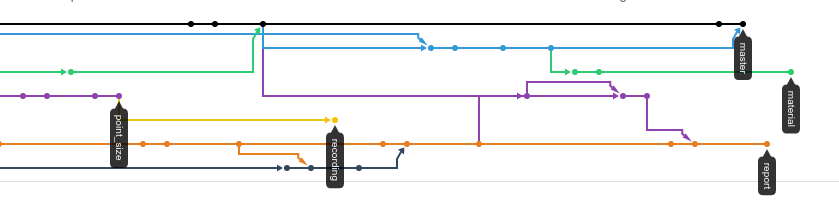
\includegraphics[scale=0.5]{github}
  \caption{Branch techniques from GitHub}
  \label{fig:github}
\end{figure}
\\
\subsubsection{Task Board}
We found a Kanban-style board very useful to help us manage tasks throughout the project. We chose to use a web platform called Trello for this, as it allowed for all team members to view and edit the board anywhere, as well as providing all the tools we were looking for. We classified each task in to three lists, one labeled "Queued" for tasks that have been planned but not started, then "In progress" for tasks that are currently being worked on, and a list for tasks that had been finished, called "Complete". We would assign these tasks to team members during our meetings, then update the status of the task as we worked on it. We aimed to keep the amount of "In progress" tasks as low as possible, focusing on finishing tasks that were semi-completed before moving on to something new. Trello would automatically notify team members when their tasks had been updated, which allowed us to effectively stay updated with the state of the project between meetings. 
\begin{figure}[h]
  \centering
  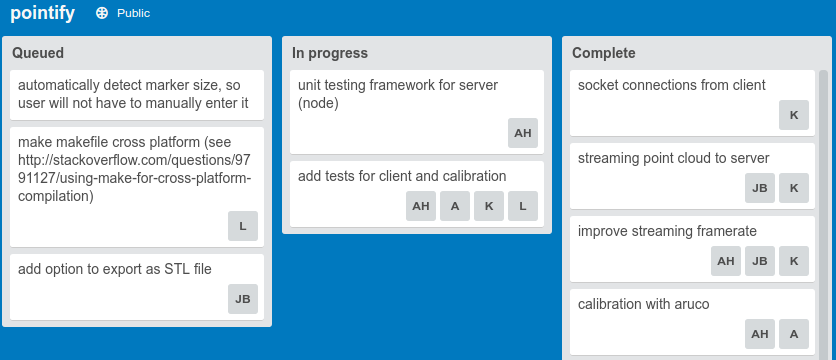
\includegraphics[scale=0.5]{trello}
  \caption{Trello project management board}
  \label{fig:trello}
\end{figure}
\\
\subsubsection{Continuous Integration and Deployment}
As our project involved building a client/server style system, we wanted somewhere that was able to constantly run the server to help when developing and demonstrating the tool. We used the Department of Computing's CloudStack instance for this, because of it's easy availability and powerful resources. 
\\\\
We wanted to spend as little time as possible manually running automated tests and following deployment processes, so we decided to use a continuous integration and deployment tool to automate this for us. We chose TeamCity as our tool, as it integrated well with our GitHub repository, and would run in the background of our deployment server. TeamCity would listen for pushes to the master branch of the GitHub repository, then try to build the code and run all automated tests over it. If all these steps were successful, and all the tests passed, we would push the changes to the deployment instance, which would be available to anyone in the college. This proved to be very useful when a single member was testing the functionality of the client software, as it required a connection to the server to run, so having a persistent instance of the server available at all times was essential. 
\begin{figure}[h]
  \centering
  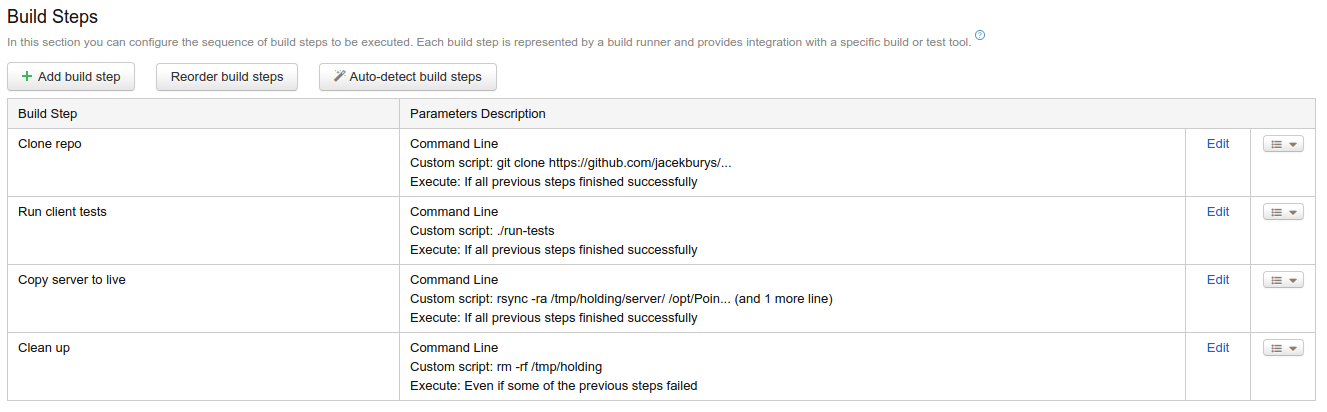
\includegraphics[scale=0.35]{buildserver}
  \caption{TeamCity build and deployment process}
  \label{fig:buildserver}
\end{figure}
\\ 
\subsection{Team Meetings}
As our project involved a lot of interaction between different parts of the code base, we had to meet often in order to discuss how this would work. We aimed to hold formal group meetings weekly, to update the team on our progress and allocate tasks for the next week, as well as meet with our supervisor to demonstrate our progress and listen to his advice. The meetings helped us keep track of what each team member was doing, as well as giving us insight into when specific parts of the project would be completed. We also held more frequent meetings during the week to discuss specific tasks that needed collaboration, and sometimes work on important features together, in a pair programming environment to ensure their quality. 
\subsection{Task Allocation}
After we had investigated the task in more detail, and understood exactly what was needed of us, we were in a position to allocate tasks to group members inside our trello board. The main tasks involved building the client system, the server system, working with the ArUco calibration library and ensuring the software could be built cross platform. We informally assigned team members to these tasks, with each member putting most of their focus on to their task. From these general aims, we would break them down into more specific tasks, such as "Improve frontend playback framerate". We tried to write our tasks such that each of them would give a real benefit to the end user, and improve their experience with the product.
\begin{figure}[h]
  \centering
  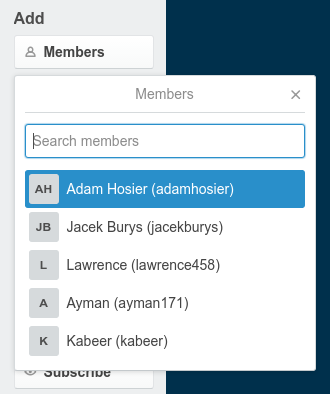
\includegraphics[scale=0.5]{trello2}
  \caption{Trello task allocation}
  \label{fig:trello}
\end{figure}
\\ 
\newpage
\subsection{Issues}
\subsubsection{LiveScan}
LiveScan is run solely on Windows and uses Visual Studio with Microsoft Kinect SDK 2.0. This posed us many problems as a group because only 3 of the members of the group used Windows systems. We also had a problem that with one of the computers, the version of Windows was the 'N' edition of the operating system. Athough we tried the recommended fixes on the internet, we were unable to get LiveScan to run on this version of Windows due to errors about missing MSVCP120.dll and MFPlat.dll. This meant that only 2 computers were able to run the LiveScan software which meant there was only one client and one server running. This did not allow us to test the feature of multiple calibrated cameras and also hindered our development that we were only able to work on 2  computers.
\\\\
We also found it difficult to work with the codebase provided by LiveScan as the quality of the code was poor and did not utilise OpenCV for matrix operations nor did it use any of the leading calibration techniques. This resulted in code that was highly fragile and highly coupled which posed us issues when we were trying to perform tasks like replacing the calibration system.
\subsubsection{Pointify}
When we opted to pivot the project and work on Pointify, we were able to alleviate a lot of the issues that we encountered when working with LiveScan. We did however have issues that we encountered during development. When we initially started development, we needed to start development on a single operating system. We chose to begin development on Linux but this meant that we needed to dual boot our computers or run Linux through a virtual machine. This meant that we were not able to begin development immediately due to the time it took to ensure that our systems were set up correctly. This also posed issues of speed when it came to processing power and networking speeds that were crucial during the development of the system. With virtual machines we were only able to allocate partial amounts of our resources to it, restricting the performance inside the operating system, this was also a problem with networking as the virtual machine uses NAT translation to control the networking within the virtual machine which hindered the network contributing to latency and therefore lag in the streaming. Another problem that we faced with the NAT translation was jitter which caused a delay with each individual packet affecting the obtained frame rate. 
\\\\
There were also hardware issues that we had to deal with. We had designed the system to be able to work with multiple cameras and calibrate them correctly. We however for the project were only provided with two kinect cameras to develop with. For testing with the picture taking, we were able to use the cameras in different positions in order to emulate how the system would be able to deal with multiple cameras. This was a sufficient method to be able to test how the calibration would be able to cope and how the rendering was able to cope with a large volume of points. For live streaming however this proved to be much more difficult. We were unable to test how the system would be able to cope with multiple cameras sending data at once and how this would affect the framerate. The fact that we needed to use the hardware to test the system was also a problem that we faced which meant that we were only able to work on the project when we were in university rather than being able to do any work remotely. For testing purposes we set the build server to be a persistent server for Pointify as well which allowed us to test the client in isolation without having to use a seperate machine to act as the server for our distributed system. We had a problem with USB 3.0 ports as well, some of the computers that we were trying to use did not have USB 3.0 which is required for \texttt{libfreenect2} drivers to be able to communicate with the camera.
\newpage
\section{Design}
We designed the project as a distributed system which has one server and multiple clients. We decided to do it like this to allow for further usability in the future if the user decides to use multiple cameras in a space and also to improve the extensibility of the product for potential new developers who may wish to create different types of clients which is possible with a standard interface.
\subsection{SocketIO}
We decided to use SocketIO to communicate between the clients and the server as it provides a simple to use decorator to the underlying networking code. This allows us to create an abstraction away from the underlying network code as well as allowing a standard interface if in the future alternative clients wish to be developed. SocketIO also has a C++ client as well as a JavaScript client which meant that we did not need to consider the networking protocols for dealing with the sockets between the server and the client. When calibrating, the server simply sends a calibration request to the client which then sends back a boolean callback if the calibration was successful or not. When streaming, the server simply requests a picture from each client every frame and synchronises the recieved frames itself so that all the client needs to do is implement one function to take a picture and does not need to know whether it is streaming or not. The server also sends start streaming and stop streaming notifications over SocketIO so that the client can change its state when streaming if required. This is done to aid further extensibility.
\subsection{Distributed System}
We chose to design our system as a distributed system for a few main reasons. Using a distributed system is good for applications like these because when adding more devices to the system, you are also adding more computers and computing power. This means that increased number of cameras has a negligible increase on the load of the server which makes the system more powerful. Another advantage of this design is that the cameras do not need to be physically connected to a single computer and can be situated in different corners of the space. This is a vital feature for some of the use cases of our system, such as imaging a point of interest which would require the cameras to be quite far from each other. There are also drawbacks of the distributed approach however. Having a computer dedicated to each camera means that the hardware requirements are greater and having the system run over the network means that the framerate and latency will be worse than having it all run on one server.
\begin{figure}[h]
  \centering
  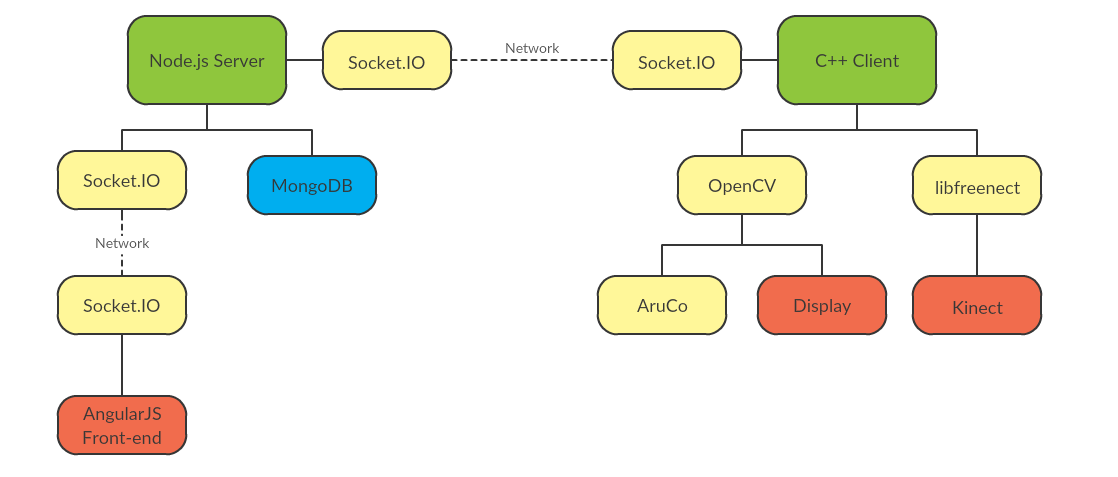
\includegraphics[scale=0.35]{distributed}
  \caption{Diagram of the distributed system design of the project}
\end{figure}
\newpage
\subsection{Client}
The UML sequence diagram of the client's structure is shown below:
\begin{figure}[h]
  \centering
  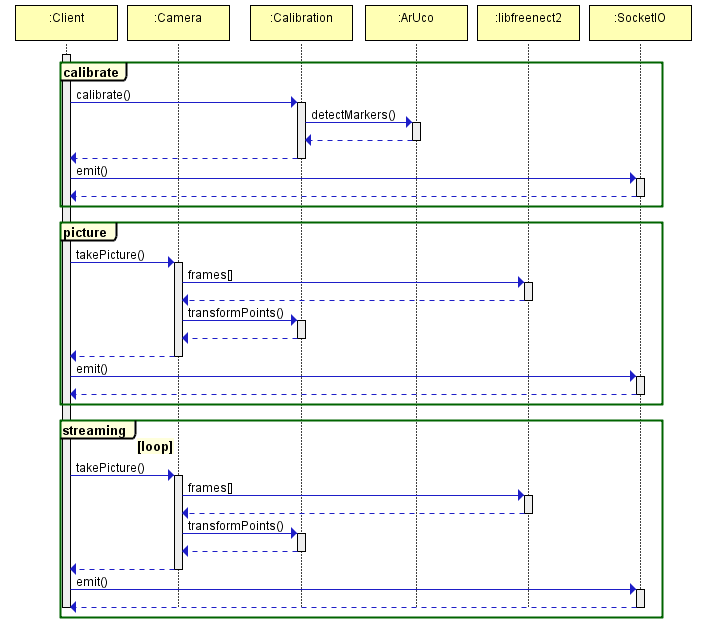
\includegraphics[scale=0.6]{clientUML}
  \caption{UML sequence diagram of the client}
\end{figure}
\subsubsection{C++}
\subsubsection{ArUco}
\subsubsection{Libfreenect}
\subsubsection{CMake}
Our tool of choice for building the client was CMake, as it is a well established tool for building cross platform applications. CMake allowed us to write one make script "CMakeLists.txt", which compiled to a build solution that would run on the user's platform. On Unix systems this would be a Makefile, which allowed to user to use "make" to build the application, and on Windows machines this compiled a Visual Studio solution which could be built inside Visual Studio. We had to make sure that the libraries we used were built for the platform that the client was running on, this could be done by building them from source inside our CMake file, or providing the users with precompiled binaries for them. For our needs we found it easier to compile the libraries to the platforms we were using, and downloading them onto the machines we worked on. 
\subsubsection{Data}
We chose to do the calibration on the server and send the point clouds directly to the client to allow for distributed computation and speed up the transfer of data.
\subsection{Server}
The UML sequence diagram of the server's structure is shown below:
\begin{figure}[h]
  \centering
  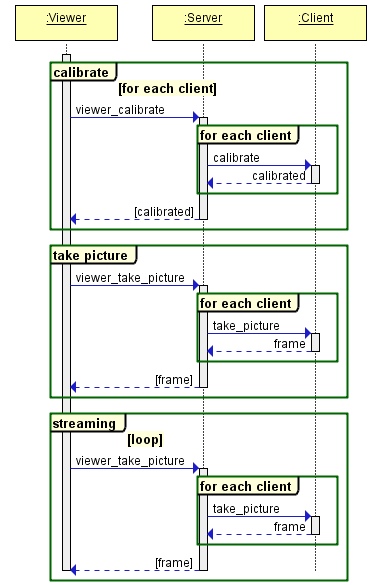
\includegraphics[scale=0.6]{serverUML}
  \caption{UML sequence diagram of the server}
\end{figure}
\subsubsection{Gulp} %webapp
\subsubsection{AngularJS}

\newpage
\section{Implementation}
\subsection{Calibration}
\subsubsection{Marker pose estimation}
When streaming with more than one camera, we required the point clouds they send to be aligned such that they can be displayed seamlessly on top of each other, building a 3 dimensional representation of the scene. The idea behind this involves applying a transformation to each point in the scene, to bring it from the camera's perspective to some common perspective shared by all the cameras. We discussed two ways of doing this, one of which chooses one of the cameras as the "master" camera, then synchronises the other cameras around it. The alternative method is by centering all of the cameras on a common point, in our case the calibration marker we use. An advantage of using the first method is that one less camera would need to be calibrated, as all of the other cameras would be centered around the master, but this would lead to more complicated code, and more difficult communication between the cameras. The second approach would give more elegant and maintainable code, as each of the cameras performs the same calibration, but sacrificing a small amount of efficiency on one of the cameras. For these reasons, we chose to use the second approach, calibrating all cameras around the marker placed in the scene. \\
\begin{figure}[h]
  \centering
  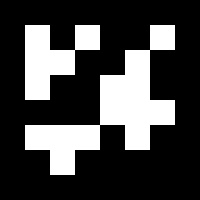
\includegraphics[scale=0.6]{aruco}
  \caption{Example ArUco marker}
\end{figure} \\
This involved working with a third party library called ArUco, which is a well established computer vision library for C++ that helps with the calibration process. In the method we chose, the cameras are all centered around a stationary marker (similar to Figure \ref{fig:aruco}) placed in the scene, so we required ArUco to detect these markers and calculate the camera's position relative to the marker. The aim is to find the transformation that brings points centered around the camera, into a space with the marker as the origin, then once this is calculated we can apply this transformation to each point cloud to align them. We start this process by detecting any markers visible in the scene, then finding rotation and translation vectors from the camera to this marker, adjusting for intrinsic camera parameters such as focal length and principal point offset. From this we can build up a transformation matrix to combine both the rotation and translation, before inverting it to get the translation from camera to marker as shown in Figure \ref{fig:transformationMatrix}. \\
\begin{figure}[h]
  \[\left(\begin{array}{cccc}
      & | &   & | \\
    - & r & - & t \\ 
      & | &   & | \\
    0 & 0 & 0 & 1
    \end{array}\right)^{-1}\]
  \caption{Transformation matrix, where \textbf{r} is the rotation and \textbf{t} is the translation}
  \label{fig:transformationMatrix}
\end{figure}

\subsubsection{Point cloud transformation}
Once we have found the transformation matrix as in the previous part, we must apply it to each point cloud before they are is sent to the server. Each xyz point must be extended with a 1 on the bottom row, so that it can be multiplied correctly with the transformation matrix. We experimented applying the transformation matrix to each point to give the transformed point, but this was causing some performance issues due to the amount of points needed to be transformed at once. A better way of doing this would be to apply the transformation to all points in one operation with a more complex matrix operation, shown in Figure \ref{fig:transformationMatrix}. We used an optimised implementation of this in opencv called perspectiveTransform to do this efficiently, which when given the set of input points, and the transformation function we calculated earlier, would return the transformed points we needed. When each client calculated the transformation to bring their origin to the marker, and applied this transformation to the point clouds captured from the connect, they could be successfully combined such that they would align.\\
\begin{figure}[h]
  \[\left(\begin{array}{cccc}
      & | &   & | \\
    - & r & - & t \\ 
      & | &   & | \\
    0 & 0 & 0 & 1
    \end{array}\right)^{-1}
  \left(\begin{array}{cccc}
    \multirow{3}{*}{\textbf{$p_1$}} & \multirow{3}{*}{\textbf{$p_2$}} & \multirow{3}{*}{\dots} & \multirow{3}{*}{\textbf{$p_n$}} \\
    & & & \\
    & & & \\
    1 & 1 & & 1
    \end{array}\right)\]
  \caption{Transformation matrix as before, applied to each point $p_1$ \dots $p_n$}
  \label{fig:transformationApplication}
\end{figure}
\newpage
\subsection{Challenges}
\subsubsection{Dual Camera Sensors}
When performing the calibration we noticed that the calibration was slightly off. After doing some research we worked out that this was caused by the offset between the depth and rgb cameras on the Kinect hardware. The reason for this was that we were performing the AruCo calibration on the rgb matrix from the colour camera and then we were using the obtained rotation and translation vectors to calibrate the output from the depth camera. This slight offset caused the obtained origin in the coordinate space to be different and then caused the point clouds obtained from the different cameras to not align correctly. This is demonstrated in figure~\ref{fig:rgbdepth} below.

\begin{figure}[h]
  \centering
  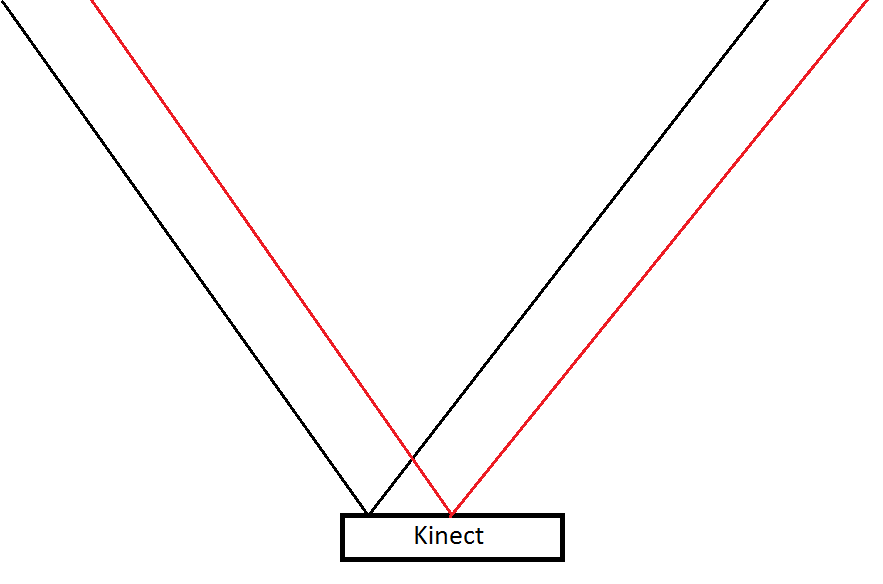
\includegraphics[scale=0.7]{rgbdepth}
  \caption{Showing the offset between the field of view of rgb and depth cameras on the Kinect}
  \label{fig:rgbdepth}
\end{figure}
This produces an offset in the calibration as shown in figure~\ref{fig:calibrationoffset} below.
\\
\begin{figure}[h]
  \centering
  
\includegraphics[scale=0.3]{placeholder}
  \caption{Showing the difference between the calibration accuracy of registered and unregistered}
  \label{fig:calibrationoffset}
\end{figure}
\\
To fix this issue we needed to use the registered camera matrix from the \texttt{apply} function within \texttt{libfreenect2}. This gave us a matrix which provided the rgb data points mapped onto the corresponding points from the depth camera's field of view. We therefore performed the calibration from the depth cameras field of view and output the correct resultant rotation and translation vectors for the point cloud generated from this camera.
\newpage
\subsubsection{Calibration Accuracy}
When using the registered matrix, we encountered a much worse camera matrix than the one directly taken from the rgb camera as shown in figure~\ref{fig:registeredaccuracy} below.
\begin{figure}[h]
  \centering
  
\includegraphics[scale=0.3]{placeholder}
  \caption{Showing the difference between the registered and rgb matrices}
  \label{fig:registeredaccuracy}
\end{figure}
\\
This reduced quality meant that AruCo was unable to accurately detect the markers in the scene. To rectify this we noticed that where \texttt{libfreenect2} was unable to detect the marker accurately, there were very small parts of the screen that were being detected as a marker as well as the main marker. This caused us issues as with multiple markers on the screen, when performing the calibration, AruCo may take the wrong marker to calibrate on, causing the points to be calibrated on the wrong location. To rectify this, during the calibration step, if there were more than one marker in the scene we would calculate the size of the 3D planes and then keep only the largest plane and remove the smaller ones. This would then return us with only the main marker in the scene if it was detected correctly.
\subsection{Unsolved Challenges}
There were also a few unsolved challenges that we face with the project that we have been unable to find a solution to at this time. These challenges that we face are related to the streaming capability of our system and they are related to the obtainable frame rate of the streaming.
\subsubsection{TCP vs UDP}
With the network we had a major problem with the protocols of TCP vs UDP. Since we are streaming the frames, UDP is a much more desirable protocol to be using to increase the framerate of our system. The first problem we encountered with using this is that SocketIO only supports TCP communication. We then considered using standard networking protocols rather than SocketIO for the streaming of the frames between the client and the server but we realised that, for the server to communicate between its nodeJS backend and its angularJS frontend, it needs to use JavaScript for the rendering of the point clouds. JavaScript as a language does not natively support UDP therefore we realised that even if we would be able to communicate the server and the client, we would encounter a bottleneck between the backend and the frontend of the server and experience no additional improvement on the framerate.
\subsubsection{Synchronisation Lag}
Lag is another issue we encountered. We were able to obtain a moderate framerate between the server and the client for streaming but we experienced on average a 3-second delay between the camera display on the client and the server. We have not found any bottlenecks within our system that could be causing this lag and we are assuming that it is simply the network delay that is causing it.
\newpage
\subsubsection{Socket.io C++ Client}
The TCP based streaming protocol that it uses has not been implemented with the current C++ client offered.
We were also experiencing problems with the network queues on the socket.
\newpage
\section{Evaluation}
\subsubsection{Design}
\subsubsection{Code Quality}
\subsubsection{Calibration Accuracy}
\subsubsection{Testing}
\subsubsection{Build Server}
\subsubsection{Deployment} %gulp
\subsubsection{Streaming}

\newpage
\section{Conclusion and Future Extensions}
\subsection{Conclusion}

When we received the proposal for 3D reconstruction, even though it was our last choice, we were nevertheless extremely excited to develop the application despite most of our members having no experience in using OpenCV. It was a great opportunity to utilise the Computer Vision materal for those in group who were taking the course because we were able to use the techniques taught and apply them in the creation of Pointify. Ensuring software development practices such as pair programming were maintained throughout the project was one of the primary importances as members are able to discuss their problems together and discuss how they could better implement a solution.
\\\\
The technical aspect of creating Pointify (coming from the idea that an object or a scene can be reconstructed by rendering many points together from captured depth information) took the most time during the 3 months. In order to start we had to understand how LiveScan3D worked which took some time as we felt that LiveScan3D's code was poorly structured. However after analysing LiveScan3D's implementation, several methods were proposed through our group meeting and then a final concrete solution was decided. We then were able to carefully plan out the major sections of the project to which each group member was assigned a task. During this short time we have endured and have managed to produce a stable application, that combined various technologies together such as angularJS and nodeJS, to successfully capture depth information through multiple Kinect cameras, perform calibration and then render the many points together to 3D reconstruct a scene. 
\\\\
Given the chance to start the project again from the beginning, we would have gone for creating the project on Linux, as it is easier to develop on there, after experiencing first hand the challenges of building the project on Windows as some time we lost was spent trying to develop on Windows. We took a risk to start afresh and develop Pointify on Linux for a cross platform application. We underestimated the complexity of the calibration of the Kinect cameras and did not consider the offset between the depth and rgb camera until our supervisor, Ben, pointed it out to us. It would have been more effective and time efficient to meticulously plan the calibration aspect of the project. The latter part of the project was spent on debugging and trying to increase the current frame (add more here)
\\\\
Overall, we are happy about the project we created over term even though we would have liked to have some of the feature extensions integrated. We have decided to release it as an open source project on github with detailed instructions on how to build, test and develop Pointify. It would be nice if we could get feedback through reported bugs as other developers may want to use Pointify in their own projects.

%What did you learn? What might you have done differently?
%How would you build on what you have done?
%As various challenges e.g. with differences in
%coordinate systems used internally by our devices and the OpenCV library code have %shown us, it would
%be wiser to first plan the procedure with finer detail. Moreover, we have been %overly focused on correctness
%of the system for a while and neglected the efficiency of the calibration phase. We %have experienced firsthand
%that the usability is crucial as the compression techniques (e.g. using %zlib_compressor class from
%boost library) were introduced quite late and our development was pointlessly slowed down.
\newpage
\subsection{Future Extensions}
There are features that we believe can improve the usability of this product, but didn't implement due to the time constraint on the project. Throughout the project we came up with possible extensions to implement for Pointify:
%1. GUI implementation%
\subsubsection{GUI Implementation}
Currently, only the server has a GUI implementation in place but the client side has no GUI implementation as everything is done by command line. As it stands now, the command line outputs non-user friendly errors to the client. We can try to build up a user friendly GUI implementation on client side to ensure a smoother client experience. The current client application only opens up the camera view for the Kinect and does not display any other helpful information. We can add to the display, the current frame rate and the calibration status of the client so it does not have to check on the server machine the status (which is useful if server and client are far way - better explain this). We can try to use some platform-independent UI library to achieve this, possibly Qt.
%2. Pointify to support other camera devices%
\subsubsection{Pointify to support other camera devices}
Modifying Pointify to work not only with Kinect cameras, but with many more types of different cameras. There are other cameras, that do not require to be plugged in to a power socket, which can capture depth information so it is possible to configure Pointify to work for these cameras. The disadvantage of using Kinect cameras is that they must be plugged into a power socket which constrains the mobility of the client should they want to roam about. What we can do is to build up a layer of indirection on the hardware driver, so that the current existing calculation(calibration?) code will work with different camera implementations. We would also need to unify the data format that is passed so that we can maximise the amount of code that can be reused.
\subsubsection{Pointify installation}
In order to get Pointify to run, several prerequsites must be installed such as \texttt{Bower}, \texttt{Ruby} and \texttt{MongoDB}. With a proper simple installation set in place, we can run a single script to detect and install the aforementioned prerequsites instead of manually installing them one by one. After the prerequsites are installed, further dependancies must be installed, the \texttt{mongod} daemon must be set up in a new shell and then finally the server started by calling \texttt{gulp serve}. The installation script would then install these dependancies and then run the daemon before starting the server in a browser window.
\subsubsection{Recordings}
A very nice feature which would go with Pointify is the ability to record point cloud streams. After successfully calibrating the clients, you can then press the "Start recording" button to record a point cloud stream which then later can be played back. The server should be able save and load these point cloud streams that it records in a database. Although each frame in size is roughly a few megabytes (?), \texttt{MongoDB} should be suitable to storing the recording point cloud streams(add more here)

% TODO : references

\end{document}
